\chapter{Preliminary Assessment and Data Gathering} % Write in your own chapter title
\label{Chapter2}
GHD conducted preliminary assessment on a set of data provided by Maynilad. The data set includes a number of records on daily production and power consumption and intervention reports issued after Maynilad experienced failure/breakdown of assets.

The assessment provided a base for GHD to generate the Inspection Testing Plan (ITP) \cite{GHD2018j} aiming to gather necessary data for conducting reliability study. The ITP has been reviewed by Maynilad, together with the Work Safety Permit (WSP), prior to execution of visual inspections and testings at the site.

\section{Maynilad's data}
\label{21}
Maynilad provided a set of data as shown in Table \ref{mayniladdata}

\begin{table}[h]
	\caption{Data provided by Client.}
	\label{mayniladdata}
	{\footnotesize
		\begin{tabular}{l|p{5cm}|p{8cm}}
			\hline
			\multicolumn{1}{c|}{No.} & Data & Remarks \\ 
			\hline
			\multicolumn{1}{c|}{1} & As-built drawings & no CAD drawings, only PDF \\ 
			\multicolumn{1}{c|}{2} & Monitoring dashboard & Year 2015 to 2017 \\ 
			\multicolumn{1}{c|}{3} & CI records & None \\ 
			\multicolumn{1}{c|}{4} & Asset registry & Asset registry was incompleted as confirmed by the IAM team of Maynilad. \\ 
			\hline
		\end{tabular}
	}
\end{table}

%\subsection{Summary}
%\label{211}

\subsection{Intervention records}
\label{212}
There are no CI reports for this station. Furthermore, the most important historical data concerning specific failure of components of pumps with elapsed time is missing. Thus, the provided information is not useful for detailed reliability study on frequent failure of assets at component level. 

The problem with missing specific failure data was due to a matter of fact that Maynilad still has not come up with preventive maintenance program within the overall asset management framework. The IAM team has recently established with expectation to generate short-term, medium-term, and long-term preventive intervention program. In close discussion with Maynilad, GHD learns that Maynilad has a regular/frequent activities for check-up (e.g. monthly and quarterly), however, recorded data has not been digitalized and the data itself has not aligned well with the asset registry. 

Table \ref{interventiondata} presents highlights on intervention data on pumps.

\begin{table}[h]
	\caption{Highlight of intervention data on pumps.}
	\label{interventiondata}
	{\footnotesize
		\begin{tabular}{l|p{6cm}|p{4cm}}
			
			\hline
			Pump & Description of PI/CI & Date/Remarks \\ 
			\hline
			All Pumps & Inspection of pump drive coupling, mechanical seal, MCC components. Conducted pump and motor vibration test using vibration meter and monitored bearing condition using thermal scanner. Also check gen-set's engine oil, radiator's coolant, battery solutions and filters. & Regular monthly maintenance activity, may vary at times depending on availability of test equipment \\ 
			Southvale P2 & Replacement of torishima pump & 6/15/2015 \\ 
			& Replacement of mechanical seal & 7/9/2015 \\ 
			& Pull-out of defective pump unit & 7/27/2015 \\ 
			Southvale P1 & Replacement of mechanical seal & 7/9/2015 \\ 
			Sonera P1 & Replacement of Element Coupling (Love joy 110) & N/A \\ 
			N/A & Installation of Pump 1 - pump and motor alignment & 4/9/2016 \\ 
			\hline
			
		\end{tabular}
		
	}
\end{table}



\subsection{Interview data}
\label{213}
GHD conducted an interview session on 07/12/2018. Results of the interview are summarized in the minutes \cite{GHD2018l}, with the following highlights.

\begin{itemize}
\item No further data is available aside from the provided set presented in earlier section;
\item There is an existing regular check-up for assets but data is not digitalized and the information is only generic;
\item Spare parts are not stocked for most of components, except for bearing. Regarding service delivery, the required discharge pressure remains the top priority in pump operation modulation and sequencing. Critical parts and components for VFD and bearing are usually stacked to have spared in case of emergency repair and replacements. The consumables on the other hand, are not stacked but ordered in advance for use in maintenance activities;
\item No visual bank of assets;
\item No standard testing regime that follows a regular scheme based on optimality;
\item Pumps are operated based on pressure and not manual;
\item No existing PI/CI procedure to be followed;
\item No expansion plan is forecasted; physically impossible to add another pump in the existing pump room
\item There is a problem with the inflow of incoming water, leading to lower level of reservoir chambers that has affected pump operations occasionally;
\item no historical data on pump efficiency, which is a simple yet useful value in determining pump performance. The main impediment in  the individual pump efficiency is the measurement of flow produced by each pump. The existing configuration of the pump-motor and piping system do not cater to conventional methods of flow determination;
\item No intervention records for FDAS. It was revealed that different version on operation and functionality of the FDAS was reported by both guard and site operators.
%\item 
\end{itemize}

\subsection{Asset hierarchy}
\label{214}
During the bidding phase, Maynilad did provide the first draft of the Asset Registry (AR) that describes a hierarchy of eight (8) levels. Figure \ref{ch02_assethierachy} visualizes the hierarchy with brief description presented in Table \ref{ch02_tbl_assethierachy}.

\begin{figure}[!htb]
	\includegraphics[scale=1.3]{figures/ch02_assethierarchy} \\
	\caption{Asset Hierarchy}
	\label{ch02_assethierachy} 
\end{figure}

\begin{table}[h]
	\caption{Condition state definition - Multiple.}
	\label{ch02_tbl_assethierachy}
	{\footnotesize
\begin{tabular}{l|p{10cm}}
	\hline
	\multicolumn{1}{c|}{Asset hierarchy} & Description \\ 
	\hline
	\multicolumn{1}{c|}{Level 1} & Stakeholder level. For example, an pump station belongs to MWSI \\ 
	\multicolumn{1}{c|}{Level 2} & Geographical locations/ or administrative zone (e.g. a pump station belong to Quezon city or Makati) \\ 
	\multicolumn{1}{c|}{Level 3} & System (e.g. the entire pump stations and reservoir system) \\ 
	\multicolumn{1}{c|}{Level 4} & Sub-system (e.g. one specific pump station and reservoir such as the Lamesa PSR) \\ 
	\multicolumn{1}{c|}{Level 5} & Functional system (e.g. booster system or storage system) \\ 
	\multicolumn{1}{c|}{Level 6} & Component (e.g. Suction line, Reservoir line and Tank) \\ 
	\multicolumn{1}{c|}{Level 7} & Sub-component (e.g. Suction pipe and fittings, Concrete reservoir, pump) \\ 
	\multicolumn{1}{c|}{Level 8} & Items (e.g. valve, bearing, motor) \\ 
	\hline
\end{tabular}		
	}
\end{table}

GHD received the latest version of the AR with about 100 assets for this PS. The full list of assets is given in the excel file provided by Maynilad in 2018. GHD has developed a MS Access program to convert the data in the excel file to a relational database structure. Per agreement with Maynilad, GHD will only verify level 7 of the AR with the actual site condition for the study \cite{GHD2018m}. 
\section{Preliminary assessment}
\label{22}
Assessment on the latest provided intervention records reveals that the provided pertinent data is incomplete and cannot be used as representative data for a complete reliability study. 

It is also confirmed from the provided data that the Client has done regularly check-up on GENSETs to ensure that it provides adequate level of services in case of emergency. To date, no failure records has been observed for the GENSET.

Further evaluations and tests have to be conducted to identify the areas for improvement of preventive measures in mitigating corrective measures and study the ways to strengthen preventive measures to improve operating conditions and life of pump components. 

Improving the reliability of the pump stations for the next coming years require evaluation of the existing pump station conditions and maintenance practices, particularly assessment of the pump and its components. With that, areas for improvement of operation and maintenance be addressed through action items that come from the resulting recommendations.

In order to capture a relatively good picture on the reliability of the pump system and its associated assets, a number of tests shall be conducted. 

\section{Summary of the inspection test plan (ITP)}
\label{231}
A complete write-up on testing shall be referred to the ITP \cite{GHD2018j}, which has been submitted, reviewed, and approved by the Client. This section only provides highlights to help readers keeping abreast  of the flow of the report.

\subsection{Mechanical Audit}
\label{232}
The Mechanical Tests to be conducted are enumerated and discussed hereunder including their background and applications, standards used if applicable, and the equipment to be used. During testing, the following are the assumptions and considerations:

\begin{itemize}
\item The operation of the pumps cannot be interrupted (at day time when demand is high).
\item The valve settings then cannot be adjusted to produce different flow rates.
\end{itemize}

\subsubsection{Structural Inspection for Pump Discharge and Suction Line}

This activity measures the current thickness of the existing pipelines at the pump vicinity using ultrasonic thickness gauging. The flow regime especially around the elbow and possibly corrosion and scaling conditions are to be predicted from the measurements of this test.

Following procedures will be executed

\paragraph{Step 1: Locate and mark testing points}
At a minimum of two (2) meters away from the pump intake/discharge flange, the test points shall be marked at 3, 6, 9 and 12 o’clock positions and at one (1) meter interval along the pipes, additional test sections with same set points shall be added as long as available beneath the immediate ground level.


%The test points shall also consider elbows on probable points of most thinning from turbulent water flow.

\paragraph{Step 2: Prepare test point surfaces}
\begin{itemize}
\item	Wipe the surface free of dirt (no need to remove paint)
\item	Using a chalkstone (erasable), mark x on the test point
\end{itemize}

\paragraph{Step 3: Apply sufficient couplant on test point surface}
\begin{itemize}
\item	Use petroleum jelly/Vaseline as couplant
\end{itemize}

\paragraph{Step 4: Set transducer probe on test point}

\paragraph{Step 5: Read and record value as indicated on module display} 


\paragraph{Step 6: Clean test point after reading}

\subsubsection{Unit Flow Measurement}
The activity measures pump capacities. Pump efficiency is then calculated using the measured values.  

\paragraph{Step 1: Locate Sensor Position Point Area and mark all points to be taken.}

\begin{itemize}
	\item Observe required offset distance from fittings/pump to consider the fully developed flow. At least 10 times the diameter distance away from the suction/discharge of the pump if applicable, otherwise consider at least 2D distance away from the fittings. This is to ensure the flow will be stable and fully developed for flow measurement accuracy %(Figure \ref{ch02_flowmeasurement01}).
	\item Otherwise, test at near turbulent zones and consider normalizing the flow. 
\end{itemize}

In particular, the headers can be chosen as set points for flow measurement. (Figures \ref{fig_ch02_ufm} - a to d).

\begin{figure}[ht]
	\begin{minipage}[b]{0.225\linewidth}
		\centering
		\includegraphics[width=\textwidth]{figures/fig_ch02_ufm3}
		\caption*{a}
		%		\label{ch02_flowmeasurement01}
	\end{minipage}
	\hspace{0.05cm}
	\begin{minipage}[b]{0.225\linewidth}
		\centering
		\includegraphics[width=\textwidth]{figures/fig_ch02_ufm4}
		\caption*{b}
		%		\label{ch02_flowmeasurement02}
	\end{minipage}
	\hspace{0.05cm}
	\begin{minipage}[b]{0.225\linewidth}
		\centering
		\includegraphics[width=\textwidth]{figures/fig_ch02_ufm1}
		\caption*{c}
		%		\label{ch02_flowmeasurement02}
	\end{minipage}
	\hspace{0.05cm}
	\begin{minipage}[b]{0.225\linewidth}
		\centering
		\includegraphics[width=\textwidth]{figures/fig_ch02_ufm2}
		\caption*{d}
		%		\label{ch02_flowmeasurement02}
	\end{minipage}
	\caption{UFM testing points}
	\label{fig_ch02_ufm}	
\end{figure}


\paragraph{Step 2: Pipe Specification Input on the Flow Meter.}
\begin{itemize}
\item Identify nominal pipe size with equivalent parameters such as schedule designation, equivalent thickness, OD, and etc.
\item Input outside diameter.
\item Input pipe thickness.
\item Input pipe material (carbon steel).
\item Input pipe medium (water).

\end{itemize}

\paragraph{Step 3: Prepare test point surfaces}
\begin{itemize}
	\item Clean the surface of pipe with a sandpaper and steel brush or any suitable abrasive materials, exposing the base metal.
	
\end{itemize}

\paragraph{Step 4: Install transducers at set points}
\begin{itemize}
	\item Apply enough couplant that it covers transducers sensors to ensure an acoustically conductive connection to the pipe. Also apply couplant on the test point surface %(Figure \ref{ch02_flowmeasurement03}).
	\item Clamp the transducers at the side of pipe using metal chains, straps or mounting rails Observing proper spacing and alignment. Note flow direction and install transducers at either 0 or 45 degrees, whichever would give more stable reading %(Figure \ref{ch02_flowmeasurement04}, Figure \ref{ch02_flowmeasurement05}, Figure \ref{ch02_flowmeasurement06})
	\item Wait for the module to display “System Normal” before reading. Inspect set-up for any fault and properly reinstall if signal is poor/low (no reading)
\end{itemize}


\paragraph{Step 5: Data gathering}
Read and record all necessary data measurement by the equipment, (i.e. flow, fluid velocity, sound velocity, Reynolds number, etc.) 

\begin{figure}[!htb]
	\includegraphics[scale=1.3]{figures/fig_ch02_flowmeasurement07} \\
	\caption{UFM Measurement Display}
	\label{ch02_flowmeasurement07} 
\end{figure}

\paragraph{Step 6: Remove transducers and restore paints}
Remove the transducers and restore the surface of pipe after measurement.

\subsubsection{Suction and Discharge Pressure Measurement}
The activity measures each pump suction and discharge pressure. The pump efficiency is then calculated using the measured values.

\paragraph{Step 1: Disassembly of existing Pressure Gauge}
\begin{itemize}
\item Inspect for any leaks or unusual noise before proceeding: If anything is detected, report immediately to the operator;
\item 	Close gate valve located before the pressure gauge and wait for the pressure reading to drop;
\item 	Remove the pressure gauge: (1) Hold the adapter steady with one wrench and the grip the stationary socket of the pressure gauge with another; (2) Loosen the pressure gauge then remove it.
\end{itemize}

\paragraph{Step 2: Installing the Pressure Gauge}
\begin{itemize}
\item Prepare the connections: (1) Clean the connections before installing; (2) Put Teflon tape on the pressure connection of the gauge;
\item Install the pressure gauge: (1) Mount the pressure gauge on the adapter then hand tighten the arrangement; (2) Further tighten the assembly using a pair of wrenches: hold the adapter steady with one wrench and the grip the stationary socket of the pressure gauge with another; (3) Tighten the assembly;
\item Inspect the assembly again.
\end{itemize}
\paragraph{Step 3: Reading the pressure}
\begin{itemize}
\item Slowly open the gate valve: Observe any leaks or unusual noise;
\item Measurement: (1) Wait until reading is stable; (2) Record the pressure as indicated.
\end{itemize}

\paragraph{Step 4: Restoring the earlier gauge}
\begin{itemize}
\item Inspect for any leaks or unusual noise before proceeding: If anything is detected, report immediately to the operator;
\item 	Close gate valve located before the pressure gauge and wait for the pressure reading to drop;
\item Remove the pressure gauge: (1) Hold the adapter steady with one wrench and the grip the stationary socket of the pressure gauge with another; (2) Loosen the pressure gauge then remove it;
\item 	Prepare the connections: (1) Clean the connections before installing; (2) Put Teflon tape on the pressure connection of the gauge;
\item 	Install the pressure gauge;
\item 	Mount the pressure gauge on the adapter then hand tighten the arrangement;
\item 	Further tighten the assembly using a pair of wrenches: hold the adapter steady with one wrench and the grip the stationary socket of the pressure gauge with another;
\item 	Tighten the assembly.
\end{itemize}
\subsubsection{Parameters}
Parameters was recorded using visual inspection form, interview questionnaire, and testing results. Main parameters are listed, but not limited to, in the Table \ref{ch02_tbl_parameter}. Raw data is enclosed in the Appendix.

\begin{table}[h]
	\caption{Main parameters to be collected.}
	\label{ch02_tbl_parameter}
	{\footnotesize
\begin{tabular}{l|l|l}
	\hline
	Parameters & \multicolumn{1}{c|}{Symbol} & Remarks \\ 
	\hline
	Pipe thickness Gauge & \multicolumn{1}{c|}{t} & \multicolumn{1}{c}{mm} \\ 
	Pump Capacity & \multicolumn{1}{c|}{Q} & \multicolumn{1}{c}{Gpm/cmh} \\ 
	Suction Pressure  & \multicolumn{1}{c|}{Ps} & \multicolumn{1}{c}{mH2O} \\ 
	Discharge Pressure & \multicolumn{1}{c|}{Pd} & \multicolumn{1}{c}{mH2O} \\ 
	Vibration Data  & \multicolumn{1}{c|}{-} & \multicolumn{1}{c}{-} \\ 
	Head & \multicolumn{1}{c|}{H} & \multicolumn{1}{c}{mH2O} \\ 
	Efficiency  & \multicolumn{1}{c|}{e} & \multicolumn{1}{c}{\%} \\ 
		\hline
	\end{tabular}		
	}
\end{table}


%\subsection{Electrical Audit}
%\label{233}
%Nam to write based on the ITP
%\subsection{Fire protection and safety (FDAS) audit}
\label{234}
It was confirmed at site that there is no FACP and the devices are only battery operated smoke detectors "KIDDE" brand. 

This smoke alarm warning device is a “stand-alone” system in which device detects and measure smoke particles and emits an audible sound but is not connected to any of the manual call point and bell that were installed separately in the pump station. There is no monitoring panel to tell where the zone/ area of the fire is and also the exact location of the fire. Table \ref{ch02_tbl_fdas01} lists major assets of the FDAS.

\begin{table}[h]
	\caption{Main parameters to be collected.}
	\label{ch02_tbl_fdas01}
	{\footnotesize
	\begin{tabular}{l|l|l}
		\hline
		Assets & Quantity & Unit \\ 
		\hline
		Smoke detectors & \multicolumn{1}{c|}{8} & \multicolumn{1}{c}{pcs} \\ 
		Call points & \multicolumn{1}{c|}{2} & \multicolumn{1}{c}{pcs} \\ 
		Bell sounder & \multicolumn{1}{c|}{2} & \multicolumn{1}{c}{pcs} \\ 
		\hline
	\end{tabular}
	}
\end{table}

The Emergency and fire fighting equipment consists of the following :
\begin{itemize}
\item Fire extinguishers Dry Chemical (Red color)
\item Fire extinguishers HCFC (Green color)
\item Emergency lighting 
\item Exit signages
\item Exit Doors
\item PPE cabinet
\item Fire hose cabinet
\item Evacuation plan for every floor
\end{itemize}

FDAS audit was conducted in the period from October 30, 2018 to November 16, 2018.


Audit on FDAS has been conducted following sequences

\paragraph{Step 1: Assign (1) one person on the Fire Alarm Control Panel  to operate / accept  the fire alarm activation and another group/person to conduct spraying on the device, communicate using two way radio.}

\paragraph{Step 2: Conduct spray of smoke detector tester (SOLO brand or any) directly on the smoke detector device for not more than 1 sec, repeat action until detector is activated. Note : If detector fails to respond after 3 tries,  device will declared faulty (Figure \ref{ch02_fdas}-a).}

\paragraph{Step 3: Hear and visually check strobe light and sounder every time you activated the smoke detectors.}

\paragraph{Step 4: Remove device and clean, allow particles to disperse. Then return to socket (Figure \ref{ch02_fdas}-b).}

\paragraph{Step 5: Check that strobe light is functioning/ blinking after returning. Note original status if no light is visible. Check that the control panel breaker feeding the device is reset (Figure \ref{ch02_fdas}-c).}

\paragraph{Step 6: Repeat steps 2, 3, and 4 on different locations until all the devices are tested.}

\paragraph{Step 7: Conduct testing for manual call point /manual pull station by pressing the device, hear if the alarm bell / buzzer is activate after you trigger the device (Figure \ref{ch02_fdas}-d).}

\paragraph{Step 8: Check bells and buzzer audibility.}

\paragraph{Step 9: Return Manual Call Point /Manual Pull Station on stand by position. Repeat it on all device.}

\paragraph{Step 10: Make a record for the fault device.}

\paragraph{Step 11: Record the status of FACP and reset the panel until the fault clear on trouble.}

\paragraph{Step 12: Conduct closing of activities to all concerned .}

\begin{figure}[h]
	\begin{minipage}[b]{0.22\linewidth}
		\centering
		\includegraphics[width=\textwidth]{figures/ch02_fdas01}
		\caption*{(a)}
		%		\label{ch02_fdas01}
	\end{minipage}
	\hspace{0.05cm}
	\begin{minipage}[b]{0.22\linewidth}
		\centering
		\includegraphics[width=\textwidth]{figures/ch02_fdas02}
		\caption*{(b)}
		%		\label{ch02_fdas02}
	\end{minipage}
	\hspace{0.05cm}
	\begin{minipage}[b]{0.22\linewidth}
		\centering
		\includegraphics[width=\textwidth]{figures/ch02_fdas03}
		\caption*{(c)}
		%	\label{ch02_fdas03}
	\end{minipage}
	\hspace{0.05cm}
	\begin{minipage}[b]{0.22\linewidth}
		\centering
		\includegraphics[width=\textwidth]{figures/ch02_fdas04}
		\caption*{(d)}
		%	\label{ch02_fdas04}
	\end{minipage}
	\caption{FDAS testing}
	\label{ch02_fdas}
\end{figure}

\subsection{Vibration and structural assessment}
\label{235}
This activity measures the vibrations of the pump and motor at the drive and non-drive ends. The data will be used to address pump vibration problems such as cavitation, pump flow pulsation, bent pump shaft, pump impeller imbalance, shaft misalignment and bearing problems.

Following procedures will be executed

\paragraph{Step 1: Test location identification}

Locate the testing points on drive and non-drive ends of pump and motor %(Figure \ref{ch02_vibrationtest01}).

\paragraph{Step 2: Set transducer probe on test point. Observe HIRAC for access to elevated positions}
\paragraph{Step 3: Read and record value as indicated on module display (Figure \ref{fig_ch02_vib} - d)}


\begin{figure}[ht]
	\begin{minipage}[b]{0.225\linewidth}
		\centering
		\includegraphics[width=\textwidth]{figures/fig_ch02_vib2}
		\caption{a}
		%		\label{ch02_flowmeasurement01}
	\end{minipage}
	\hspace{0.05cm}
	\begin{minipage}[b]{0.225\linewidth}
		\centering
		\includegraphics[width=\textwidth]{figures/fig_ch02_vib3}
		\caption{b}
		%		\label{ch02_flowmeasurement02}
	\end{minipage}
	\hspace{0.05cm}
	\begin{minipage}[b]{0.225\linewidth}
		\centering
		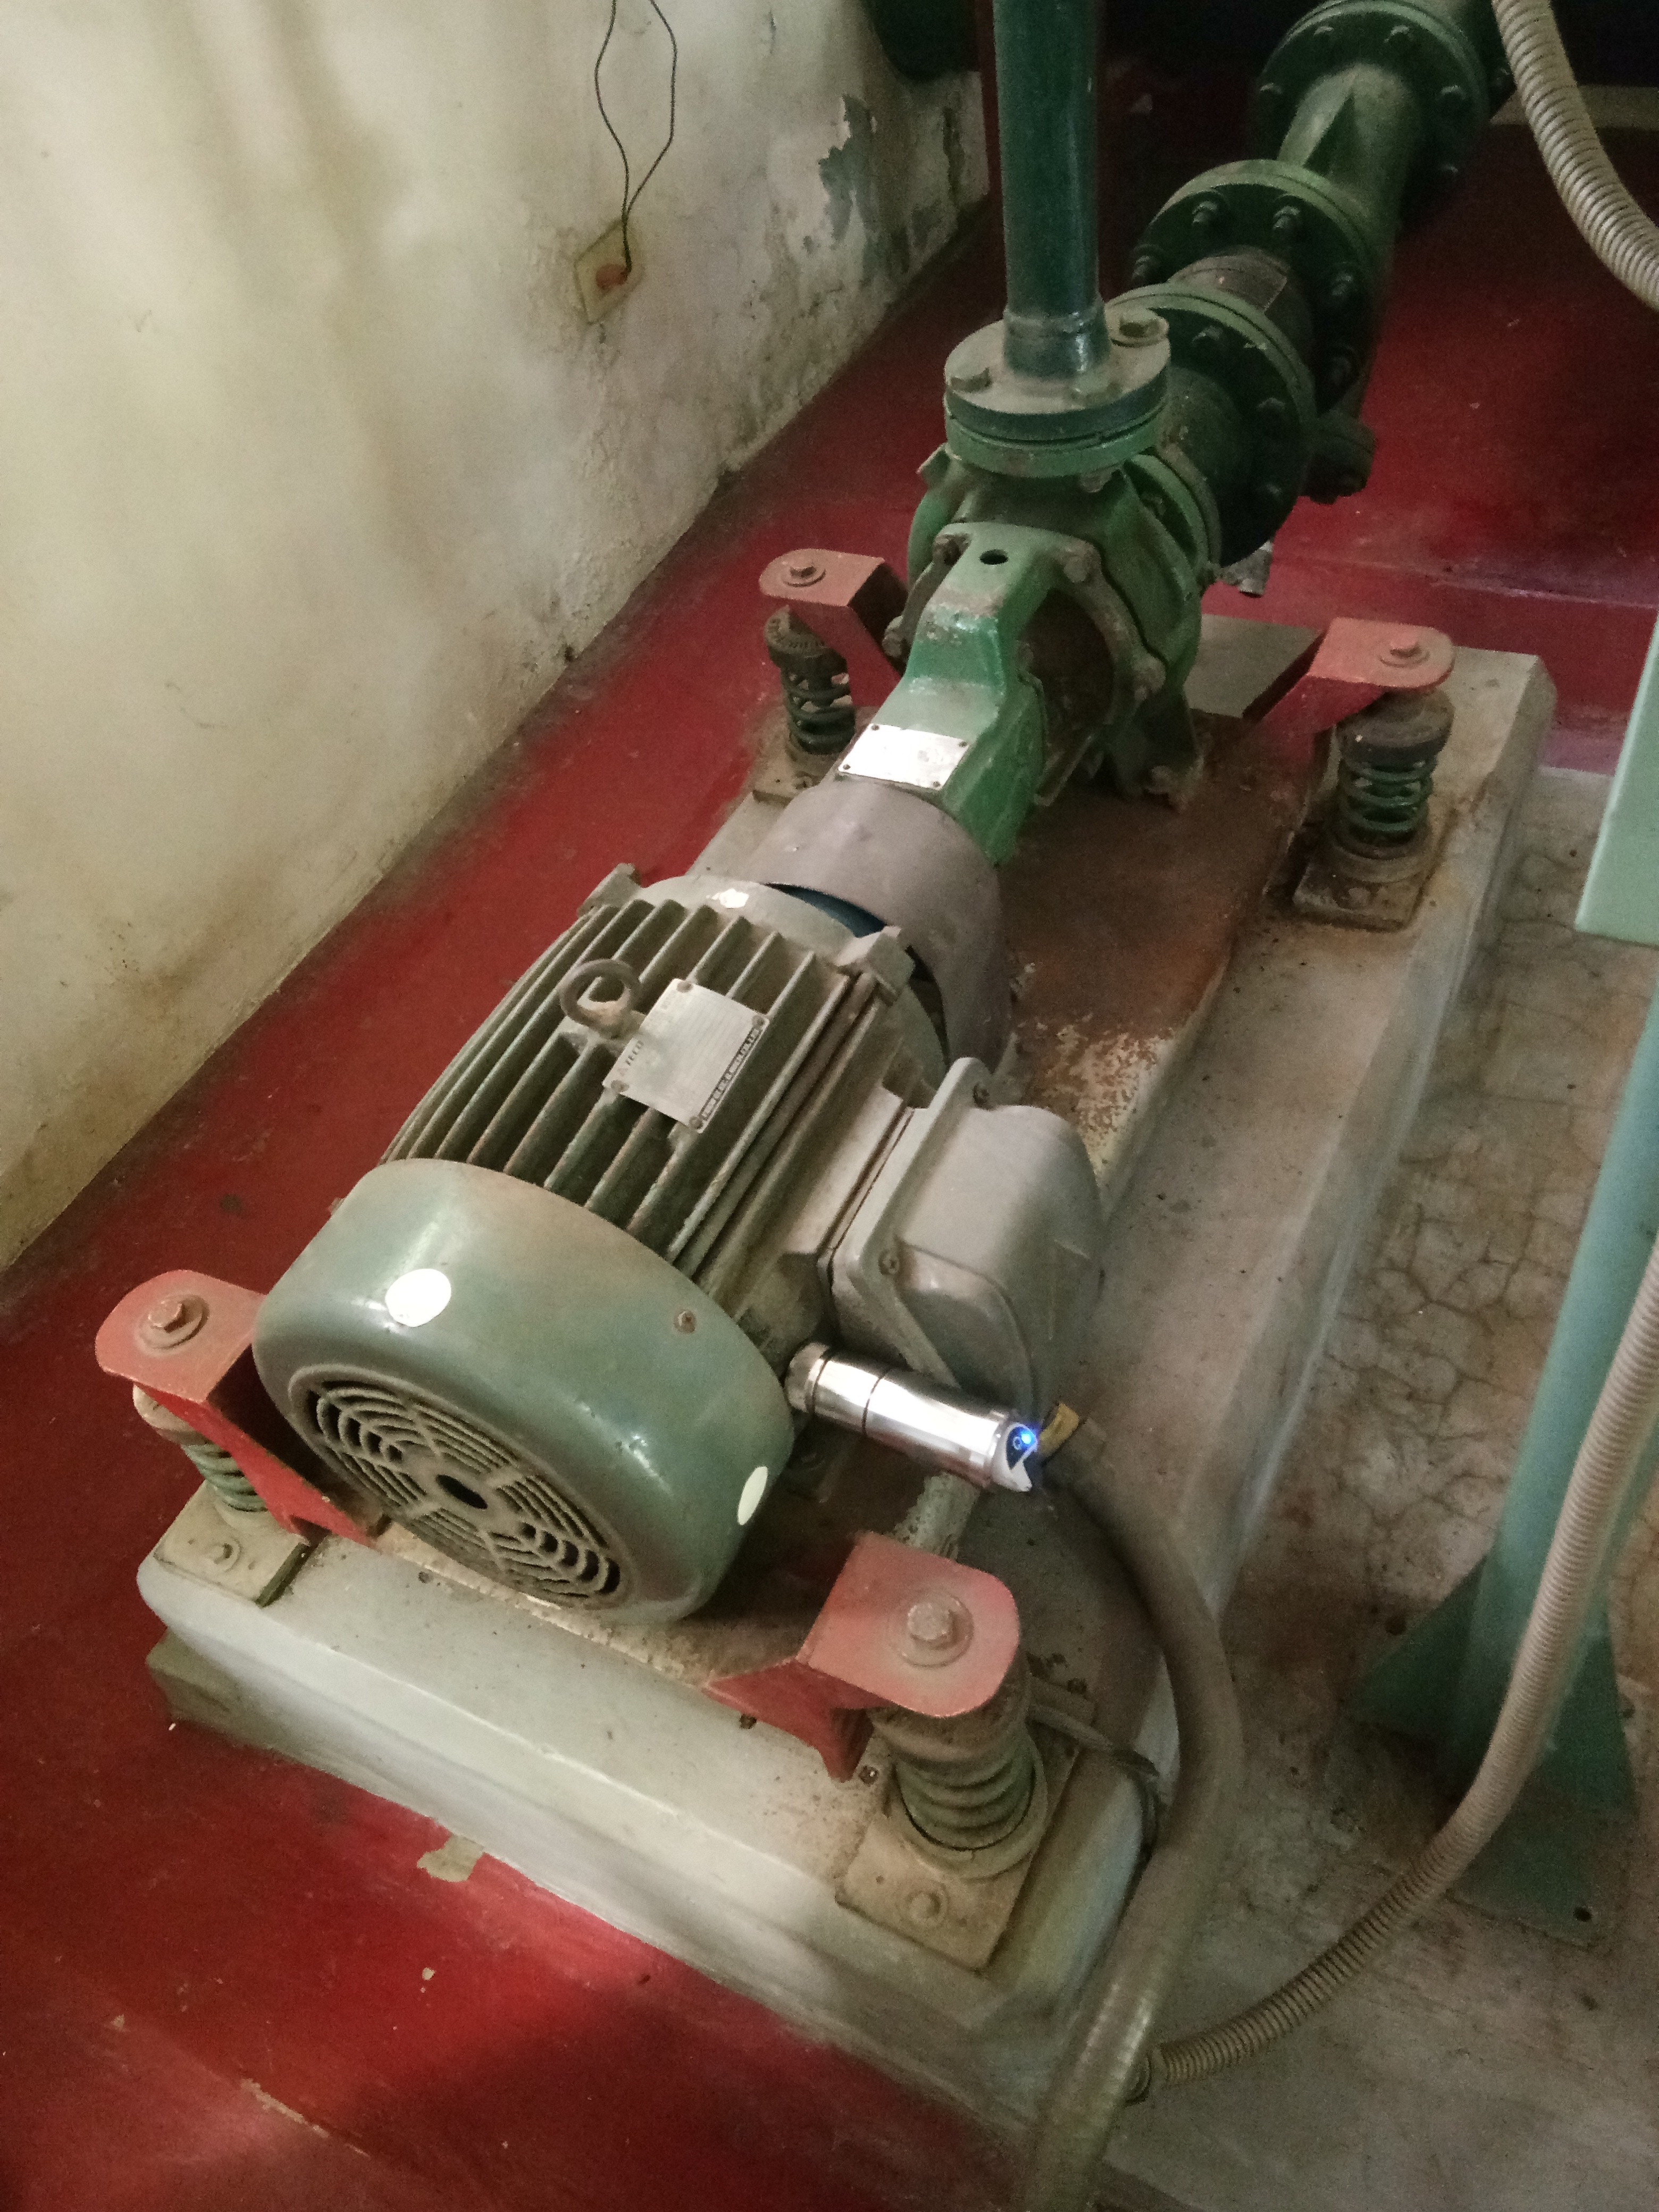
\includegraphics[width=\textwidth]{figures/fig_ch02_vib4}
		\caption{c}
		%		\label{ch02_flowmeasurement02}
	\end{minipage}
	\hspace{0.05cm}
	\begin{minipage}[b]{0.225\linewidth}
		\centering
		\includegraphics[width=\textwidth]{figures/fig_ch02_vib1}
		\caption{d}
		%		\label{ch02_flowmeasurement02}
	\end{minipage}
	\caption{Vibration Analyzer Test}
	\label{fig_ch02_vib}	
\end{figure}


\subsection{Workplace environment management}
\label{237}

GHD/RBSanchez conducted measurements at designated locations (Figure \ref{fig_ch02_wem01}) to record values of parameters presented in Table \ref{ch02_tbl_wemparameter}.

\begin{figure}[!htb]
	\includegraphics[width = \textwidth]{figures/fig_ch02_wem01} \\
	\caption{Testing locations}
	\label{fig_ch02_wem01} 
\end{figure}

\begin{table}[h]
	\caption{WEM Parameters.}
	\label{ch02_tbl_wemparameter}
	{\footnotesize
		\begin{tabular}{l|l|l}
			\hline
			Parameters & \multicolumn{1}{c|}{Symbol} & \multicolumn{1}{c}{Units} \\ 
			\hline
			Dry Bulb Temperature & \multicolumn{1}{c|}{tdb} & \multicolumn{1}{c}{oF/oC} \\ 
			Relative Humidity & \multicolumn{1}{c|}{RH} & \multicolumn{1}{c}{\%} \\ 
			Sound Intensity & \multicolumn{1}{c|}{-} & \multicolumn{1}{c}{dB} \\ 
			PM 2.5 Count & \multicolumn{1}{c|}{PM2.5} & \multicolumn{1}{c}{$ug/m^3$} \\ 
			Visible useful light & \multicolumn{1}{c|}{-} & \multicolumn{1}{c}{Lux} \\ 
			\hline
		\end{tabular}	
	}
\end{table}


\subsection{Fire protection and safety (FDAS) audit}
\label{234}
It was confirmed at site that there is no FACP and the devices are only battery operated smoke detectors "KIDDE" brand. 

This smoke alarm warning device is a “stand-alone” system in which device detects and measure smoke particles and emits an audible sound but is not connected to any of the manual call point and bell that were installed separately in the pump station. There is no monitoring panel to tell where the zone/ area of the fire is and also the exact location of the fire. Table \ref{ch02_tbl_fdas01} lists major assets of the FDAS.

\begin{table}[h]
	\caption{Main parameters to be collected.}
	\label{ch02_tbl_fdas01}
	{\footnotesize
	\begin{tabular}{l|l|l}
		\hline
		Assets & Quantity & Unit \\ 
		\hline
		Smoke detectors & \multicolumn{1}{c|}{8} & \multicolumn{1}{c}{pcs} \\ 
		Call points & \multicolumn{1}{c|}{2} & \multicolumn{1}{c}{pcs} \\ 
		Bell sounder & \multicolumn{1}{c|}{2} & \multicolumn{1}{c}{pcs} \\ 
		\hline
	\end{tabular}
	}
\end{table}

The Emergency and fire fighting equipment consists of the following :
\begin{itemize}
\item Fire extinguishers Dry Chemical (Red color)
\item Fire extinguishers HCFC (Green color)
\item Emergency lighting 
\item Exit signages
\item Exit Doors
\item PPE cabinet
\item Fire hose cabinet
\item Evacuation plan for every floor
\end{itemize}

FDAS audit was conducted in the period from October 30, 2018 to November 16, 2018.


Audit on FDAS has been conducted following sequences

\paragraph{Step 1: Assign (1) one person on the Fire Alarm Control Panel  to operate / accept  the fire alarm activation and another group/person to conduct spraying on the device, communicate using two way radio.}

\paragraph{Step 2: Conduct spray of smoke detector tester (SOLO brand or any) directly on the smoke detector device for not more than 1 sec, repeat action until detector is activated. Note : If detector fails to respond after 3 tries,  device will declared faulty (Figure \ref{ch02_fdas}-a).}

\paragraph{Step 3: Hear and visually check strobe light and sounder every time you activated the smoke detectors.}

\paragraph{Step 4: Remove device and clean, allow particles to disperse. Then return to socket (Figure \ref{ch02_fdas}-b).}

\paragraph{Step 5: Check that strobe light is functioning/ blinking after returning. Note original status if no light is visible. Check that the control panel breaker feeding the device is reset (Figure \ref{ch02_fdas}-c).}

\paragraph{Step 6: Repeat steps 2, 3, and 4 on different locations until all the devices are tested.}

\paragraph{Step 7: Conduct testing for manual call point /manual pull station by pressing the device, hear if the alarm bell / buzzer is activate after you trigger the device (Figure \ref{ch02_fdas}-d).}

\paragraph{Step 8: Check bells and buzzer audibility.}

\paragraph{Step 9: Return Manual Call Point /Manual Pull Station on stand by position. Repeat it on all device.}

\paragraph{Step 10: Make a record for the fault device.}

\paragraph{Step 11: Record the status of FACP and reset the panel until the fault clear on trouble.}

\paragraph{Step 12: Conduct closing of activities to all concerned .}

\begin{figure}[h]
	\begin{minipage}[b]{0.22\linewidth}
		\centering
		\includegraphics[width=\textwidth]{figures/ch02_fdas01}
		\caption*{(a)}
		%		\label{ch02_fdas01}
	\end{minipage}
	\hspace{0.05cm}
	\begin{minipage}[b]{0.22\linewidth}
		\centering
		\includegraphics[width=\textwidth]{figures/ch02_fdas02}
		\caption*{(b)}
		%		\label{ch02_fdas02}
	\end{minipage}
	\hspace{0.05cm}
	\begin{minipage}[b]{0.22\linewidth}
		\centering
		\includegraphics[width=\textwidth]{figures/ch02_fdas03}
		\caption*{(c)}
		%	\label{ch02_fdas03}
	\end{minipage}
	\hspace{0.05cm}
	\begin{minipage}[b]{0.22\linewidth}
		\centering
		\includegraphics[width=\textwidth]{figures/ch02_fdas04}
		\caption*{(d)}
		%	\label{ch02_fdas04}
	\end{minipage}
	\caption{FDAS testing}
	\label{ch02_fdas}
\end{figure}

\section{Electrical Audit}
The detail of the electrical audit testing procedure is presented in the Inspection Testing Plant (ITP) \cite{GHD2018j}, which has been submitted to Maynilad along with the WSPs and were approved prior to the execution of tests.

\section{Database}
\label{24}
GHD developed an MS Access program that functions as a database used to record data collected from visual inspections and testings. The database has been developed using the concept of Relational Database Management System (RDMS), which is a must to record data systematically. The benefits of using the database are

\begin{itemize}
	\item Eliminate redundancy and repetition of same data
	\item Eliminate incorrect data entry that is often found when working with excel files
	\item Provide linkages among asset hierarchy
	\item Provide ease for programing (e.g. reliability modeling and life cycle cost analysis)
	\item Support Maynilad AIM team to learn the benefits of using RDMS in developing an integrated Asset Management System for now and future
	\item Provide compatibility with any CMMS that is often using other RDMS such as Microsoft SQL Server, Oracle SQL server, or MySQL platform
	\item Provide ease for compilation of desire tables for further analysis using SQL (Structure Query Language)
	\item Provide ease for importing/exporting to different extension formats (e.g. flat, csv, xlsx)
	\item Provide a strong background for Maynilad team to migrate recording practices to Web-based that will be part of GHD's recommendation for future usage.
\end{itemize}

The MySQL database is then migrated into MySQL server, which is powerful database system that is used also to migrate, compile, and store all production and power consumption data into a single table. Main reasons behind the development of the MySQL server are for statistical computing with R and for faster compilation of queries.

GHD will provide these two sets of database as part of our deliverable and will provide training for Maynilad team to learn how to use the database in an efficient approach.




